\section{Circular Dependency}

\examplefigfour

The circular dependency represents a cycle among a group of processes in a CTP. A deadlock occurs when a receive on each process in the cycle waits for the issuing of a send on another member process but never gets a response. 
%a message $m$ from another process, but no one is able to send its message before receiving $m$. A deadlock occurs for a circular dependency if the CTP can be scheduled such that each member process in the circular dependency arrives at a receive that is not able to be matched with a send on another member process. 

The circular dependency in \defref{def:circular} is from the definition of lock dependency \cite{DBLP:conf/pldi/JoshiPSN09}. It depends on the sequential relation in \defref{def:seqrelation}. 

\begin{definition}
A sequential relation for a process, $p$, is a three-tuple $(p, \mathit{r_c}, \mathit{s_l})$, where the receive $\mathit{r_c}$ and its nearest-enclosing wait are both followed by the send $\mathit{s_l}$ on $p$. 
\label{def:seqrelation}
\end{definition}

\begin{definition}
Given a set of sequential relations, $D$, a circular dependency $\tau$ $=$ $\langle(p_0, \mathit{r}_0, \mathit{s}_0),$ $\ldots,$ $(p_m, \mathit{r}_m, \mathit{s}_m)\rangle$ is a sequence in $D$, such that the following properties hold.
\begin{compactenum}
\item at least two sequential relations exist in $\tau$;
\item for all integers $i,j \in [0,m]$, $p_i \neq p_j$, i.e., the processes $p_0$, $p_1$, $\dots$, $p_m$ are all distinct objects;
\item for all $i \in [0,m]$, $j = (i+1) \% m$, the send $\mathit{s}_i$ can potentially match the receive $\mathit{r}_j$;
%\item for all $i \in [1,m]$, if $\mathtt{r}_i$ is a deterministic receive, then there are no wildcard receives preceding $\mathtt{r}_i$ on $p_i$.
\end{compactenum}
\label{def:circular}
\end{definition}

In \figref{fig:deadlock2}, the CTP has a circular dependency in messages $\langle(p_0, \mathit{r_{0}}, \mathit{s_{1}}),$ $(p_1, \mathit{r_{2}}, \mathit{s_{2}}),$ $(p_2, \mathit{r_{3}}, \mathit{s_{3}})\rangle$ that may cause the CTP to deadlock. For instance, $\mathit{r_{0}}$ can never match $\mathit{s_{3}}$ because of the dependency. For simplicity, an instance of the circular dependency pattern only records the receives. For example, $(\mathit{r_{0}}, \mathit{r_{2}}, \mathit{r_{3}})$ is an instance of the circular dependency pattern for the CTP in \figref{fig:deadlock2}. As a note, this section considers only infinite buffer semantics in the discussion of algorithms and examples. The zero buffer semantics are discussed in section 6.


\subsection{Pattern Match for Circular Dependency}

\begin{algorithm}
\caption{Finding Circular Dependency}\label{algo:circular}
\begin{algorithmic}[1]
%\Require $\mathit{ctp}$, a single-path MPI program
%\Require $\mathit{M}(\mathtt{r_c}) = \{\mathtt{s_l}\mid(\mathtt{s_l},\mathtt{r_c})\in\mathit{M}\}$, a set of potentially matched sends for $\mathtt{r_c}$
\State $\mathit{PT} \gets \emptyset$
\State $\mathit{E} \gets \emptyset$, $\mathit{V} \gets \emptyset$
%a relation from an operation $\mathit{e}$ to another operation $\mathit{e}$
%a set of operations
\State $\mathit{R} \gets \emptyset$, $\mathit{R_w} \gets \emptyset$
%\State $\mathit{PT}$, a set of circular dependency pattern instances
%\State $\mathit{R}(p) = \{\mathtt{r_c}\mid(p,\mathtt{r_c})\in\mathit{R}\}$, the witnessed receives on process $p$
%\State $\mathit{R_w}(p) = \{\mathtt{r_c}\mid(p,\mathtt{r_c})\in\mathit{R_w}\}$, the receives for the last witnessed wait on process $p$ 
\For{$(e_1, e_2, \dots, e_n) \in \mathit{ctp}$}
\For{$i \gets 1$ to $n$}
\If{$\mathit{e_i}$ is a receive}
%\If{$\mathit{isIssued}$ and $\mathtt{e}$ is a deterministic receive}
%\State \textbf{break}
%\EndIf
%\If{$\mathtt{e}$ is a wildcard receive}
%\State $\mathit{isIssued} \gets true$
%\EndIf
\State $\mathit{R} = \mathit{R} \cup \{\mathit{e_i}\}$
\State $\mathit{V} = \mathit{V} \cup \{\mathit{e_i}\}$
\For{$\mathit{s_l} \in \mathit{M}(\mathit{e_i})$} \Comment{add match relation}
\State $\mathit{E} = \mathit{E} \cup \{(\mathit{s_l},\mathit{e_i})\}$  
\EndFor
\EndIf
\If{$\mathit{e_i}$ is a wait}
%\For{$\mathit{r_c} \in \mathit{R}$}
\State $\mathit{R_w} = \mathit{R_w} \cup \mathit{R}$
%\EndFor
\State $\mathit{R} \gets \emptyset$ 
\EndIf
\If{$\mathit{e_i}$ is a send}
\State $\mathit{V} = \mathit{V} \cup \{\mathit{e_i}\}$
\For{$\mathit{r_c} \in \mathit{R_w}$}  \Comment{add HB relation on $\mathit{r_c}$ to $\mathit{e_i}$}
\State $\mathit{E} = \mathit{E} \cup \{(\mathit{r_c},\mathit{e_i})\}$
\EndFor
\EndIf
\EndFor
\State $\mathit{R} \gets \emptyset$, $\mathit{R_w} \gets \emptyset$
\EndFor
\State $\mathit{PT} \gets$ \Call {Johnson}{$\mathit{V}$, $\mathit{E}$}
\end{algorithmic}
\end{algorithm}

\algoref{algo:circular} shows the steps for finding all the instances of the circular dependency pattern in a $\mathit{ctp}$. As a reminder, $M$ is the set of potential match pairs for the \emph{ctp}. In general, the algorithm is part of the function $\mathrm{PATTERNMATCH}$ in \algoref{algo:main}. 
It first maps a $\mathit{ctp}$ to a graph that consists of a set of vertices $\mathit{V}$ and a set of edges $\mathit{E}$. 
It then detects all the cycles in the graph based on Johnson's algorithm \cite{DBLP:journals/siamcomp/Johnson75}.
 
%In \algoref{algo:circular}, the variable $\mathit{V}$ is a set of operations. The variable $\mathit{E}$ is a set of edges each representing a relation from one operation to another. 
The set $\mathit{PT}$ stores the matched pattern instances.
The set $\mathit{R}$ stores the witnessed receives on a process that is represented as a list of operations $(e_1, e_2, \dots, e_n)$. 
The set $\mathit{R_w}$ stores the receives that are recently witnessed on $p$.
%Each process $p$ in $\mathit{ctp}$ is a list of operations $(e_1, e_2, \dots, e_n)$. 

The function $\mathit{M}(\mathit{r_c}) = \{\mathit{s_l}\mid\langle\mathit{r_c},\mathit{s_l}\rangle\in\mathit{M}\}$ returns all potential sends for the receive. The algorithm checks each operation $e_i$ in $p$. 
If $\mathit{e_i}$ is a receive, then it is inserted into $\mathit{R}$ at line 7 and is inserted into $\mathit{V}$ at line 8. 
Also, for each potentially matched send $\mathit{s_l}$ in $\mathit{M}(\mathit{e_i})$, the relation $(\mathit{s_l},\mathit{e_i})$ is inserted into $\mathit{E}$ at line 10 indicating that a match relation on $\mathit{s_l}$ to $\mathit{e_i}$ is an edge in the graph. 
If $\mathit{e_i}$ is a wait, all the receives in $\mathit{R}$ are inserted to $\mathit{R_w}$ at line 14 and $\mathit{R}$ is set back to an empty set at line 15, indicating that all the receives in $\mathit{R}$ are witnessed by $\mathit{e_i}$. 
\defref{def:seqrelation} requires for each sequential relation that the receive and its nearest-enclosing wait both precede the send on an identical process. 
Therefore, the happens-before relation (a partial order over two operations) on a witnessed receive to a following send on an identical process is considered as an edge in the graph because they can be potentially matched as a sequential relation.
As such, if $\mathit{e_i}$ is a send, the algorithm checks each witnessed receive $\mathit{r_c}\in \mathit{R_w}$ at line 19, and inserts the happens-before relation $(\mathit{r_c},\mathit{e_i})$ into $\mathit{E}$ at line 20. 

Finally, the function $\mathrm{JOHNSON}$ implements Johnson's algorithm to compute all the cycles in the graph. Since an edge in any computed cycle is either a receive-send happens-before relation on an identical process, or a send-receive match relation across two processes, there exists exactly one sequential relation for any process in the cycle. Therefore, each cycle computed by the function $\mathrm{JOHNSON}$ is an instance of the circular dependency pattern. As discussed earlier, only receives in each cycle are stored to represent an instance in the set $\mathit{PT}$. The complexity of program traversal is $O(\mathrm{N}^2)$, where $\mathrm{N}$ is the total number of operations in the program. The complexity of Johnson's algorithm is $O((|V|+|E|)(\mathrm{c}+1))$ $\approx$ $O((\mathrm{c}+1)\mathrm{N}^2)$, where $\mathrm{c}$ is the number of cycles. Therefore, the total complexity of the algorithm is $O((\mathrm{c}+1)\mathrm{N}^2)$.

\begin{figure}[h]
\centering
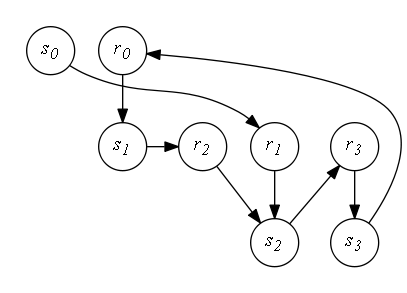
\includegraphics[scale=0.45]{fig/circulardependencyGraph1.png}
\caption{The graph built on the CTP in \figref{fig:deadlock2} by \algoref{algo:circular}.}
\label{fig:circulargraph}
\end{figure}

\figref{fig:circulargraph} shows the graph that is built on the example CTP in \figref{fig:deadlock2} by \algoref{algo:circular}. 
In the graph, the vertices include $s_0,$ $r_0,$ $s_1,$ $r_1,$ $r_2,$ $s_2,$ $r_3,$ and $s_3$. The edges include the match relations $(s_3,r_0),$ $(s_0,r_1),$ $(s_1,r_2),$ and $(s_2,r_3),$ and the happens-before relations $(r_0,s_1),$ $(r_1,s_2),$ $(r_2,s_2),$ and $(r_3,s_3)$. 
As shown in the graph, a cycle $r_0\rightarrow s_1\rightarrow r_2\rightarrow s_2\rightarrow r_3\rightarrow s_3\rightarrow r_0$ exists where the receives are stored as an instance of the circular dependency pattern.

%The completeness for \algoref{algo:circular} is given in \lemmaref{lemma:pmcircular}. 
\begin{lemma}
\label{lemma:pmcircular}
The pattern match in \algoref{algo:circular} is complete indicating that all possible pattern instances are detected (it may include some instances that do not have deadlocks).
\end{lemma}
\begin{proof}
The graph built by \algoref{algo:circular} consists of all possible vertices and all possible edges because the algorithm statically traverses each process from the beginning to the end and adds an edge once the relation is detected. Also, Johnson's algorithm is able to compute all the cycles in the graph. Therefore, all possible instances for the circular dependency pattern are detected. 
\end{proof}

\subsection{Validation for Circular Dependency}

%%revise the following algorithm of validating circular dependency pattern

If the function \textrm{FEASIBLECHECK} demonstrates that a potentially feasible schedule exists, the deadlock is further validated by (1) for the pattern instance \textit{pt}. 
\begin{equation}
\forall r_c\in \mathit{pt}(\mathit{N_s}(\mathit{dest},\mathit{src}) \leq \mathit{N_r}(\mathit{dest},\mathit{src}))
\end{equation}
where $\mathit{dest}$ is the destination endpoint of the receive $r_c$, and $\mathit{src}$ is the source endpoint of $r_c$. 
The formula checks whether there exists a send that may match any receive $\mathit{r_c}$ in \textit{pt} by comparing the count of issued sends and the count of issued receives.    
The function $\mathit{N_s}(\mathit{dest},\mathit{src})$ returns the count of issued sends with the destination $\mathit{dest}$ and the source $\mathit{src}$. The function $\mathit{N_r}(\mathit{dest},\mathit{src})$ returns the count of issued receives with the destination $\mathit{dest}$ and the source $\mathit{src}$.
%because $\mathit{r_c}$ can be matched and the cycle in \textit{pt} does not exist any more. 
If the formula is satisfied, then the algorithm detects a real deadlock for \textit{pt}.
If the formula is unsatisfiable for any receive $r_c$ in \textit{pt}, then no real deadlock exists for \textit{pt}.

The CTP in \figref{fig:nodeadlock2} is an example that has no deadlock for the circular dependency pattern instance. In \figref{fig:nodeadlock2}, process $p_0$ sends a message to $p_1$, receives a message from any source, and then sends another message to $p_1$. Process $p_1$ receives a message from any source, and then sends a message to $p_2$. Process $p_2$ receives a message from $p_1$, and then sends a message to $p_0$. As shown, the underlined commands represent an instance of the circular dependency $(r_0,r_1,r_2)$. However, (1) is not satisfied because the send $s_0$ matches the receive $r_1$ and the cycle does not exist any more. 

\begin{comment}

\begin{algorithm}
\caption{Validate Circular Dependency}\label{algo:vcircular}
\begin{algorithmic}[1]
%\Require $\mathit{ctp}$, a single-path MPI program
%\Require $\mathit{M}(\mathtt{r_c}) = \{\mathtt{s_l}\mid(\mathtt{s_l},\mathtt{r_c})\in\mathit{M}\}$, a set of potentially matched sends for $\mathtt{r_c}$
%\State  $\mathit{PT}$, a set of pattern instances
%\State  $\mathit{pt}$, a set of receives in the pattern instance $\mathit{pt}\in\mathit{PT}$
%\State $\mathit{N_s}$, a set of numbers each representing the the number of issued sends given a destination and a source
%\State $\mathit{N_r}$, a set of numbers each representing the number of issued receives given a destination and a source
%\State ($\mathit{ctp}_s, \mathit{N_s}, \mathit{N_r}, \mathit{empty}_{pt}) \gets$ \Call {ScheduleFinder}{$\mathit{pt}$}
%\If{$\mathit{empty}_{pt}$} 
%\If{\Call{isCircular}{$\mathit{pt}$}}
\For{$\mathit{r_c}\in\mathit{pt}$}
\State $\mathit{src} \gets$ source endpoint of $\mathit{r_c}$ 
\State $\mathit{dest} \gets$ destination endpoint of $\mathit{r_c}$
\If{$\mathit{N_s}(\mathit{dest},\mathit{src}) > \mathit{N_r}(\mathit{dest},\mathit{src})$}
\State report no deadlock and exit.
\EndIf
\EndFor
\State report deadlock.
%\State report deadlock and exit.
%\EndIf
%\If{\Call {isMismatch}{$\mathit{pt}} \in$}
%\If{\textproc{SAT}({\Call {Encode}{$\mathit{ctp}_s$}})}
%\State report deadlock and exit.
%\EndIf
%\EndIf
%\EndIf
%\EndProcedure
\end{algorithmic}
\end{algorithm}

\end{comment}

%%Soundness proof for pattern match needs to be added. the following proof needs to be revised to show that the validation is sound and complete.

%The soundness and completeness proof for the validation in the formula (1) is given in \lemmaref{lemma:circular}.

\begin{lemma}
The validation in (1) for an instance of the circular dependency pattern, $\mathit{pt}$, is sound and complete indicating that any detected deadlock is a real deadlock and any instance that does not satisfy (1) is a not a real deadlock. 
\label{lemma:circular}
\end{lemma}
\begin{proof}
Since the counts stored in \epsnd\ and \eprcv\ are correct (\coref{cor:count}), (1) is able to correctly check if an instance is a real deadlock or not. If the formula is unsatisfiable for some receive $r_c$, then $r_c$ can be matched and the dependency in the cycle does not exist. Therefore, $\mathit{pt}$ does not imply a real deadlock. If the formula is satisfied, then no receive in $\mathit{pt}$ can be matched. Therefore, a real deadlock occurs for $\mathit{pt}$.
\end{proof} 

%%zero buffer for circular dependency




